\part{Surfaces, Light, and Legibility}

\chapter{Materials, Lighting, and Legibility}

\section{Why Appearance Needs an Account}

Chapters 4 through 6 produced structures whose properties can be stated without any picture: a mesh with a given Euler characteristic, a family with a counted number of instances, an arrangement of nine circles with $26$ or $54$ vertices, and a network whose stocks obey a ledger. A picture of such a structure is a second object, with its own parameters and its own ways of failing, and the question of this chapter is what a picture can be made to carry and how that can be checked. The treatment is quantitative throughout. Materials assign colours and reflectance to surfaces, lights supply energy that the surfaces return, and a view transform maps the resulting radiance to the numbers stored in an image file. Each stage has a measurable law, and each can erase a distinction that the structure contains. The chapter's constructions are the two arrangements of Chapter 11 and the network run of Chapter 6, rendered so that multiplicity and stock can be read from the image, and its checks are those of the Centerfuge headless suite, examined for what each one establishes and what it leaves open.

All measurements below were made with Blender's Python module, version $5.2.2$, run headless, with the Eevee engine and software rendering. The Cycles engine is not included in the module build used here, so nothing below depends on it. The scenes are built by script, one datablock at a time, in the manner of Chapter 2, and the scripts are part of the evidence: a reader who doubts a number can rerun the script that produced it.

\section{What a Material Assigns}

A material is a datablock that tells the renderer what a surface does with light. In the Principled BSDF used throughout this book the relevant inputs are a base colour, a roughness, a metallic fraction, and optionally an emission colour and strength, and a material built from an Emission shader alone replaces reflection by a constant radiance. Two facts about these inputs matter for everything that follows. Colour inputs are linear: a value of $0.5$ in a base-colour field means half the incident light is reflected in each channel, which is not what an eight-bit pixel value of $128$ means. And a material is shared by reference. Assigning one material to a hundred objects creates no copies, in the same way that the shared meshes of Chapter 5 create no copies of geometry, and changing the material changes every user.

The assignment of a material to an object has two routes that behave differently once meshes are shared. A material slot linked to \emph{data} stores the material in the mesh, so every object using that mesh shows the same material. A slot linked to the \emph{object} stores the material in the object, so objects sharing one mesh can still differ. The arrangement scene below uses a single marker mesh for all vertices and sets each marker's slot to the object link, so that the multiplicity of the vertex, and with it the colour, is an attribute of the instance and the geometry is stored once. A scene of $54$ markers then contains one marker mesh and three marker materials. The conversion from the eight-bit colours used in an image to the linear values that a material wants is the standard sRGB decoding, and it is the one function a script of this kind cannot omit.

\lstinputlisting[language=Python,basicstyle=\ttfamily\footnotesize,breaklines=true,frame=single,columns=fullflexible,keepspaces=true,firstline=28,lastline=47]{arrangement_scene.py}

One portability note belongs here. The flag \texttt{use\_nodes}, which these scripts set to obtain a node tree on materials and worlds, is reported as deprecated and expected to be removed in Blender $6.0$. A script written for the present version will run and warn, and a script intended to outlive that version will need to be revised.

\section{Colour as a Code}

An image can carry two kinds of information in colour. A \emph{category}, such as the number of circles meeting at a vertex, is carried by a small set of colours chosen to be distinct from each other and from their surroundings. A \emph{quantity}, such as a stock, is carried by an ordered ramp in which the ordering of the colours reproduces the ordering of the values. Using a ramp for a category invents an order the data lack, and using a categorical palette for a quantity discards the order the data have. For the three multiplicity classes the scene uses the Okabe and Ito palette, a set designed to remain distinguishable under the common colour-vision differences: blue for $m=2$, orange for $m=3$, and reddish purple for $m=4$. For the network stocks it uses the viridis ramp, whose lightness increases monotonically from the low end to the high end, so that the ordering survives conversion to grey.

Figure 7.1 shows the repository script's arrangement of Section 11.8 and the teaching arrangement, each with markers coloured by multiplicity. The camera and lights are the same in both, the markers use an Emission shader at strength one, and the view transform is Standard, which maps linear values to sRGB without tone compression. These choices make the colour that reaches the image the colour that was assigned, so the image can be read back as a measurement, and they are choices for measurement and not a recommendation for finished imagery.

\begin{figure}[ht]
\centering

\includegraphics[width=0.48\textwidth]{figs/fig7_source.png}\hfill

\includegraphics[width=0.48\textwidth]{figs/fig7_teaching.png}
\caption{The arrangement of the repository script (left, $26$ vertices) and the teaching arrangement (right, $54$ vertices) viewed from the same direction. Blue markers have $m=2$, orange $m=3$, and reddish purple $m=4$. In the left image the quadruple points are conspicuous and three are visible; in the right image only the north pole is.}
\end{figure}

What the image establishes about multiplicity can be tested. The scene knows which markers exist and which circles pass through each. A marker can appear in the image only if some point of its surface is reachable by an unobstructed ray from the camera, and the test uses two bounds. The \emph{centre} bound counts a marker only if the ray to its centre is unobstructed and falls inside the frame, which undercounts markers that peek around the limb of the globe or past a thin tube while their centres are hidden. The \emph{surface} bound counts a marker if any sampled point on its surface is reachable, which is the upper estimate. The image is then analysed by finding connected regions of each assigned colour. For the script's arrangement the centre bound gives $(6,2,3)$ markers of multiplicity $2$, $3$, and $4$, the surface bound gives $(8,4,3)$, and the image contains $(7,4,3)$ regions of those colours, inside the bracket in every class. For the teaching arrangement the bounds are $(20,2,1)$ and $(27,2,1)$ and the image contains $(27,2,1)$. A preliminary run showed why two bounds are needed: every marker that the centre test declared reachable was present in the image, $11$ of $11$ in the first case, while three markers were visible that the centre test missed, one at the limb of the globe and two with a thin tube grazing the centre. The centre test is therefore a sufficient condition for visibility and not a necessary one.

The comparison also shows what colour contributes beyond visibility. Rendered with one colour for all markers, the script's arrangement shows $14$ marker regions, which equals the sum of the three coded counts $7+4+3$, so the number of visible vertices is unchanged. What is lost is the assignment of any region to a class, since an observer of the uniform image can count the vertices and cannot say how many circles meet at any of them. The coded image establishes multiplicity for the visible vertices only. Of the $26$ markers in the script's arrangement $14$ appear, and the other $12$ are on the far side of the globe, so a statement such as ``the arrangement has six quadruple points'' is a statement about the model that no single view of this image can certify.

\section{The View Transform Between Assignment and Image}

A colour assigned in a material is not the colour stored in the image. Between them lie the lighting, the exposure, and the view transform, and the last of these is chosen by a setting that is easily left at its default. A direct measurement isolates it. Three flat emissive patches carry the three class colours, the world is black, and the camera looks straight at them, so the displayed value depends on the assigned colour and the view transform alone.

\begin{center}
\begin{tabular}{@{}lccc@{}}
\toprule
Condition & Blue & Orange & Purple\\
\midrule
Assigned (sRGB) & (0, 114, 178) & (230, 159, 0) & (204, 121, 167)\\
Standard, strength 1 & (0, 114, 178) & (230, 159, 0) & (204, 121, 167)\\
AgX, strength 1 & (4, 119, 169) & (197, 145, 53) & (180, 131, 157)\\
AgX, Medium High Contrast look & (0, 118, 175) & (210, 148, 35) & (191, 134, 164)\\
Standard, strength 3 & (0, 188, 255) & (255, 255, 0) & (255, 199, 255)\\
\bottomrule
\end{tabular}
\end{center}

Standard reproduces the assigned colours exactly. AgX, which is the default view transform in the version used here and the one whose look the Centerfuge suite requests, moves the orange by $(-33,-14,+53)$ in the three channels, which exceeds the per-channel tolerance of $22$ used for the regions above, so a classifier built on the assigned colours would fail under it without any change to the scene. An emission strength above one under Standard clips: orange becomes pure yellow and purple becomes a near-white pink, so that a colour intended to mean a class acquires a different hue. The scenes of the suite assign emission strengths up to $3$ and apply a tone mapper, which suits an illustration meant to look luminous and does not make colour a reliable code. The practical rule is that colour carries information in an image only when the chain from assignment to pixel has been measured, as in the table, and that a render made for appearance and a render made for reading off values are different artifacts.

\section{Light as a Model}

A light is also a model with parameters, and for the simplest case the model can be fitted from renders. Place a diffuse patch of albedo $\rho$ under a point light of power $P$ at distance $d$ along a direction making angle $\theta$ with the patch normal, with a black world so that the light is the only source. The classical law for a Lambertian surface gives a radiance proportional to $\rho P\cos\theta/d^2$, and the question is whether Blender's renderer follows it and with what constant. A set of $64\times64$ renders written as linear OpenEXR files, read from the central pixel, gives the following ratios against a reference of $1000$ watts at distance $4$ and normal incidence.

\begin{center}
\begin{tabular}{@{}lcccc@{}}
\toprule
Varied quantity & Value & Measured ratio & Law & Difference\\
\midrule
Power $P$ & 250 & 0.2481 & 0.2500 & $-0.8\%$\\
 & 500 & 0.4990 & 0.5000 & $-0.2\%$\\
 & 2000 & 2.0004 & 2.0000 & $+0.02\%$\\
 & 4000 & 4.0008 & 4.0000 & $+0.02\%$\\
Distance $d$ & 2 & 3.9932 & 4.0000 & $-0.2\%$\\
 & 3 & 1.7771 & 1.7778 & $-0.04\%$\\
 & 6 & 0.4434 & 0.4444 & $-0.2\%$\\
 & 8 & 0.2482 & 0.2500 & $-0.7\%$\\
Angle $\theta$ & $30^\circ$ & 0.8661 & 0.8660 & $+0.01\%$\\
 & $45^\circ$ & 0.7076 & 0.7071 & $+0.07\%$\\
 & $60^\circ$ & 0.5001 & 0.5000 & $+0.02\%$\\
 & $75^\circ$ & 0.2590 & 0.2588 & $+0.08\%$\\
\bottomrule
\end{tabular}
\end{center}

A straight line fitted to the logarithm of the central pixel against the logarithm of the distance has slope $-2.0036$, against $-2$ for the inverse-square law. The reference value itself is $1.2653$, and the constant $\rho/(4\pi^2)$ with $\rho=0.8$, $P=1000$, and $d=4$ gives $0.8\cdot1000/(4\pi^2\cdot16)=1.2665$, which agrees to $0.1\%$. Under these settings the observed meaning of a point light of power $P$ watts is therefore a radiance $\rho P\cos\theta/(4\pi^2d^2)$ from a Lambertian patch, and the watt is a unit of the renderer and not a radiometric power in the laboratory sense. The residual differences of a few tenths of a percent are largest at the extremes of the power and distance ranges and are small enough that the law may be used for planning, but the table reports them and does not round them away. The script \texttt{light\_law.py} reproduces it.

The law has a consequence for legibility that the three-point lighting convention, a bright key light with a fainter fill and a rim light behind the subject, only partly addresses. A pixel's value is a product of albedo, power, the cosine of the angle of incidence, and the inverse square of distance, all at once, and nothing in a single pixel separates them. A darker pixel might be a darker material, a surface turned away from the light, a surface farther from it, or a dimmer lamp. When shading is the carrier of the shape of the globe, as it is in Figure 7.1, this entanglement is wanted: the gradient across the sphere is how the eye reads curvature. When a quantity is to be read from colour, shading is a nuisance, which is why the data-carrying markers in the figures use emission. The two roles are separated by giving each its own mechanism, with lit surfaces conveying form and emissive marks conveying data.

\section{What the Suite's Checks Establish}

The headless Blender suite of the Centerfuge repository, at commit \texttt{b0648ff}, treats a render as a record that must be verified by checks before it is admitted. Three checks bear on this chapter, and for each it is useful to state both what a pass establishes and what it does not, because the vocabulary of verification invites a reading that the code does not support. The statements below come from reading the code and from controlled probes that run the suite's own functions unchanged.

\paragraph{The image check.} The function \texttt{verify\_image\_not\_degenerate} loads the rendered PNG and requires the standard deviation of a sample of its pixel values, scaled to $0$ to $255$, to be at least $1.5$. Its sample is the slice \texttt{image.pixels[::sample\_stride * 4]} with a stride of seven. The pixels of a four-channel image are stored as a flat list of floats, so a slice stepping by $28$ always lands on the same channel, the first, which is red. Probes with synthetic images confirm the consequence. A uniform dark frame fails, as intended. An image of random noise, which contains no scene at all, passes with a standard deviation of $73.4$. An image of strong green stripes with a red channel of zero fails with a measured deviation of zero, and the same stripes written to the red channel pass with $127.5$. A cyan square on a near-black background, whose red channel is constant, also fails. The check therefore establishes that the red channel of the sampled pixels varies by more than about one and a half grey levels. It does not establish that anything is drawn, that the drawing is the intended one, or that colours in the other two channels are present, and because the suite's palette is cyan, green, violet, and amber, whose red components are low for two of the four, the check is weaker for them than for a red object. Measured over the whole image, the four committed renders have red-channel deviations between $45.7$ and $56.9$ grey levels, so they pass with a wide margin.

\paragraph{The non-occlusion check.} The function \texttt{verify\_visibility} casts a ray from the camera to up to $24$ sampled points of each object tagged as interior, taking mesh vertices or, for curve objects, control points, and counts a point as reached if the ray meets nothing before it or if the first thing it meets is the object itself. An object passes if at least $60\%$ of its sampled points are reached, and the scene fails unless every tagged object passes. Controlled probes show its extent. A lone sphere in front of the camera scores $1.00$ although only $40\%$ of its vertices face the camera, because a ray to a far-side vertex first meets the sphere itself, and the rule counts that as success. A sphere behind the camera also scores $1.00$, because no frame test is made. A target behind an opaque wall scores $0.00$, and it still scores $0.00$ when the wall is excluded from rendering and when the wall is given a nearly transparent material, because the ray cast sees evaluated geometry and not the render's visibility flags or the material. A pass therefore establishes, for the sampled points, that no \emph{other} object's geometry lies on the straight segment from the camera origin, and it does not establish that the point is inside the frame, faces the camera, is lit, or would be drawn.

A fourth probe addresses the cutaway scene itself. Run under the version used here with rendering skipped, the scene \texttt{centerfuge\_cutaway.py} at this commit raises the check's own error before saving, with an overall reached fraction of $0.34$ and $52$ of its $71$ tagged objects below the threshold. The rotor rings average $0.57$, between $0.46$ and $0.96$, the spindle scores $0.50$, and the material packets average $0.44$ with individual values from $0$ to $1$, a spread that the housing's right-hand wall plausibly explains, since the committed render shows part of the interior hidden behind it. The spokes average $0.05$ for a structural reason: each spoke contributes only its two end points, one at the axis inside the spindle and one on the rotor ring, and the first object met on a ray to either end is the spindle or the ring and never the spoke, while the midpoint, which would be reached, is not sampled. A direct probe with one ring, one spindle, and one spoke confirms the first hits. The committed render of the scene, shown in Figure 7.2, nevertheless shows an evidently open cutaway. The discrepancy is informative and concerns the check's design and not the scene's: a per-object threshold applied to end points can reject a scene that a viewer would accept, while the same rule accepts objects behind the camera. Whether the check in this repository was exercised against its own scene before being added is not something the files show, and the committed output directory contains no manifest.

\begin{figure}[ht]
\centering
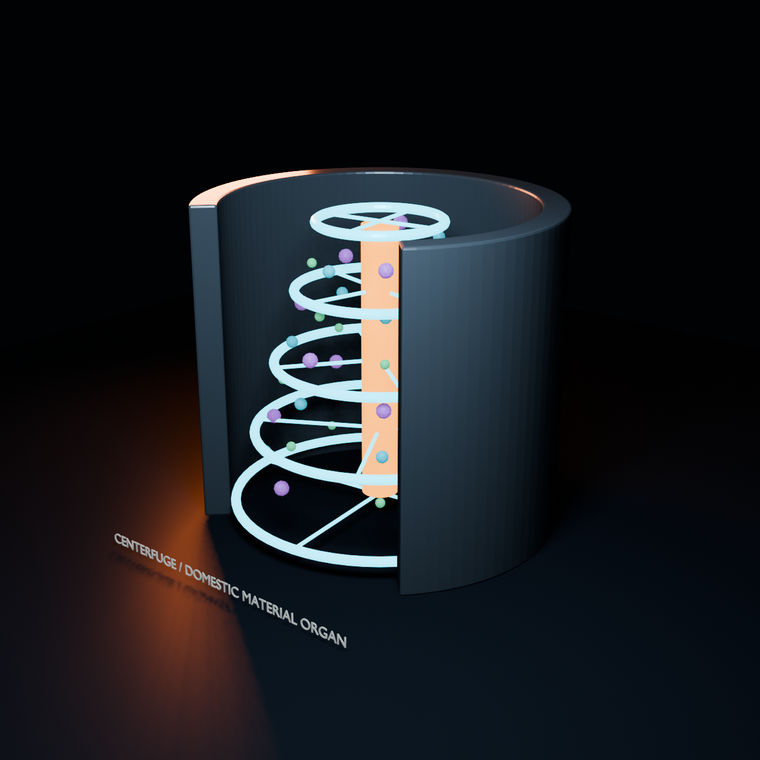
\includegraphics[width=0.52\textwidth]{figs/fig7_cutaway.png}
\caption{The cutaway render committed in the repository. The interior is plainly visible through the opening. The scene's own non-occlusion check, run as written under Blender $5.2.2$, reports a reached fraction of $0.34$ against a requirement of $0.6$.}
\end{figure}

\paragraph{The manifest check.} The script \texttt{check\_manifest.py} reads \texttt{manifest.json} and the directory listing, and it needs no Blender. It requires an entry for each of seven named scenes, the output files that the entry names, a recorded image verification for each rendered scene, and a recorded visibility verification for the two scenes that claim an interior view. This is a check on the completeness of a record: it establishes that the recorded steps were reported as having run and that the files they claim exist. It does not establish that a recorded verification was run on this code state, that its threshold is meaningful, or that the render shows what its label says. Run on the committed output directory it exits with failure, because that directory contains four scenes' files and no manifest. The separation of recording from admission, which the repository's own documents insist on, is respected in the code, and the value of the separation is exactly that the admitting step can be audited without trusting the recording one.

\begin{center}
\begin{tabular}{@{}p{0.26\textwidth}p{0.34\textwidth}p{0.32\textwidth}@{}}
\toprule
Check & A pass establishes & A pass leaves open\\
\midrule
Image non-degeneracy & The red channel of every seventh pixel varies by more than $1.5$ levels. & Any scene content; the other channels; correctness.\\
Non-occlusion & For up to $24$ sampled points per object, no other object lies on the segment from the camera. & Frame, facing, lighting, render flags, transparency; points on the object's own far side.\\
Manifest & A record exists and the files it names are present. & That the recorded checks ran on this code; that they are adequate.\\
\bottomrule
\end{tabular}
\end{center}

\section{A Check Built for the Question}

The arrangement scene of Section 7.3 performs a check designed for a stated purpose, and its structure is the one the suite's checks lack. The purpose is that a reader recover, for the visible vertices, the number of circles meeting there. The check therefore asks the image for exactly that: it detects regions of each class colour and compares their counts with two independent predictions from the scene, one a lower bound and one an upper estimate, and it reports the bracket and not a pass or fail. A conclusion drawn from it is correspondingly narrow. For the two arrangements and the one camera it establishes that colour recovers multiplicity of the visible vertices under Standard colour management; it says nothing about the other views, nothing about AgX, and nothing about the hidden vertices. The check also states a way to fail: a change of view transform moves the colours outside the detection tolerance, as the table of Section 7.4 shows.

The same pattern applies to quantities. The network run of Chapter 6 produced $121$ states of $54$ nodes, and Figure 7.3 shows three of them, at times $5$, $20$, and $120$, on three globes with a common orientation. Node colour comes from the viridis ramp applied to the stock divided by the largest stock in the whole run, $1.6869$, so the three globes are comparable and the early frames are dark by construction. That choice is deliberate: normalising each frame to its own peak would make every frame look equally saturated and would hide the growth that the sequence exists to show. Markers have a single size, so colour is the only carrier. The image was then read back. For each marker whose centre is reachable from the orthographic camera, the colour at the projected centre was matched to the nearest of the $256$ ramp colours and converted to a stock. Of the $162$ markers, $90$ are reachable by the centre ray, and $63$ of those face the camera by more than a cosine of $0.2$. For those $63$ the recovered stock is within $0.183\%$ of the peak, with a median error of $0.099\%$, which is the quantisation of a $256$-step ramp. The remaining $27$ grazing markers contain $5$ misreadings of between $4\%$ and $19\%$ of the peak. These are nodes at the limb for which the ray reports the marker as reached while the pixel at its projected centre shows a tube or the background, because most of the marker lies behind the globe. The centre-ray rule that the suite uses is therefore also not sufficient for legibility at grazing angles, and the readback is the check that detects it.

\begin{figure}[ht]
\centering
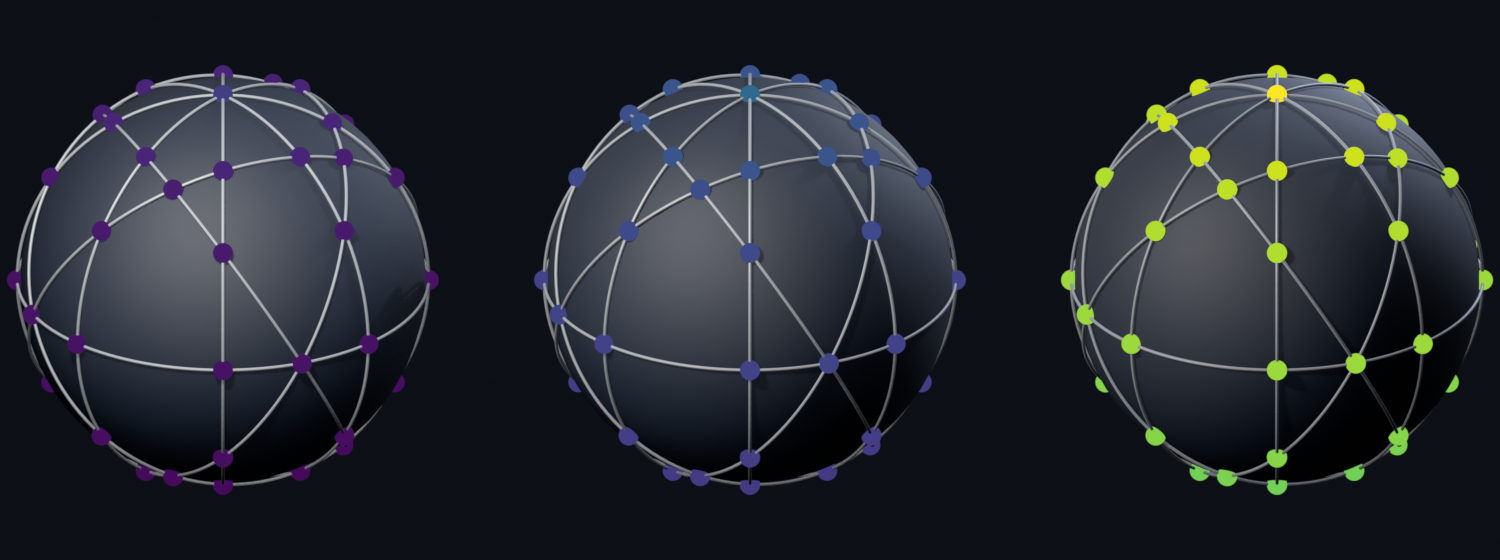
\includegraphics[width=\textwidth]{figs/fig7_network.png}
\caption{The network of Chapter 6 at times $5$, $20$, and $120$, with node colour from stock on a single ramp normalised by the peak stock of the whole run. Stock enters at the north pole, which becomes the brightest node, and spreads over the sphere. The ramp clamps stock below zero to its lowest colour, so a negative stock would be indistinguishable from zero in this image.}
\end{figure}

Two limits of the picture should be stated beside it. The ramp clamps negative stock to the bottom colour, as the Chapter 6 export script clamps negative scale, so a run that violated nonnegativity would look the same as one that did not, and the nonnegativity check of Chapter 6 must be made on the data. And a view shows about half of the nodes: $90$ of $162$ markers are reachable, and the south pole, where the drain acts, is on the hidden side in the chosen view. An animation of this kind is a presentation of a recorded run, and what it can support is a statement about visible nodes at the sampled times, resolved to the ramp's quantisation, for non-grazing nodes.

\section{Reading a Rendering Honestly}

The constructions of this chapter converge on a practice. State what the picture is meant to carry, choose a carrier suited to it, and measure that the carrier survives the chain from assignment to pixel. Colour needs a palette matched to the kind of information, an exposure and view transform that do not alter it, and a measurement of what the transform does. Shading needs a lighting model whose parameters are known, and the law $\rho P\cos\theta/(4\pi^2d^2)$ is that model for a point light in this renderer. A check on the result needs a stated purpose, and a passing check must be read for what it establishes. Ray-cast reachability, a red-channel contrast threshold, and a manifest of recorded results are each useful, and none of them is a judgment that the image is legible.

\begin{exercise}[7.1: Moving the colours]
Render the script's arrangement with the view transform set to AgX and run the colour detection with the tolerance of $22$ used in the text. State which classes are lost and by how much each channel moved. Then widen the tolerance until all three classes are recovered and check whether any two class colours can now be confused with each other or with the lit tubes. Finally choose a different measurement for the same purpose, for example a render with a flat unlit shader for the markers, and compare what each approach can and cannot say about the finished, tone-mapped image.
\end{exercise}

\begin{exercise}[7.2: A check that fits the cutaway]
Using the probe results above, design a replacement for the non-occlusion check that would accept the committed cutaway and reject an opaque shell. Decide which points to sample on curves and on the object's own surface, whether to require the points to be inside the frame, and whether the threshold should apply to each object or to the scene. Run the existing scene against your check and against the original, and write two sentences stating what your check establishes that the original does not, and what it still leaves open.
\end{exercise}

\begin{exercise}[7.3: Fitting the light]
Reproduce the table of Section 7.5 for an area light instead of a point light, varying power and distance. State the exponent you measure for distance and explain, by considering the geometry of the light's size, why it may differ from $-2$ at short range. Report the constant that replaces $1/(4\pi^2)$ for your light.
\end{exercise}
